\label{chap:rel}


\section{High Recall Information Retrieval}

High Recall Information Retrieval deals with retrieval problems where the goal
is to find all or nearly all relevant documents while maintaining a high
precision. \textit{Recall} of a retrieval system is defined as the fraction of
relevant documents it retrieved, while \textit{precision} is defined as the
fraction of retrieved documents which were relevant. Legal eDiscovery is one
such high-recall problem where all the evidence related to some matter is
required to be retrieved from a digital collection of
information~\cite{oard2013information,oard2010evaluation}. The eDiscovery
process involves lawyers reviewing documents and it is desirable to keep the
review costs reasonable by minimizing the amount of non-relevant documents
reviewed. High recall problems also extend to patent
retrieval~\cite{lupu2013patent} and systematic reviews~\cite{yu2016read} in the
medical/health space. In information retrieval, test collections are used to
evaluate and compare different retrieval systems. A test collection comprises of
a document corpus, a set of queries (or information needs) and for each query,
relevance judgments on a set of documents. To build test collections,
conferences such as the Text REtrieval Conference (TREC) employ human assessors
to manually label a fixed number of documents retrieved by multiple retrieval
systems.  Building test collections can also be interpreted as a high-recall
problem because it is desirable to find all relevant documents using fixed
amount of assessor effort.

Traditional web search systems address a different set of information retrieval
problems where the goal is to deliver a small ordered list of highly relevant
documents, which are preferably at top.  Evaluation of such systems is usually
done using the Cranfield paradigm~\cite{voorhees2001philosophy}, using metrics
such as precision at certain ranks, MAP (Mean Average Precision), nDCG
(Discounted Cumulative Gain), and so on. Such retrieval systems and evaluation
techniques usually favour early precision and cannot be directly used in the
context of high recall retrieval~\cite{magdy2010pres,roegiest2017design}. In
addition to measuring recall, it is important to factor in the effort spent by
the user when evaluating high recall systems. The search tasks in many high
recall applications are complex and even the user's understanding of the task
requirements may change during the search process. Some systems used for high
recall tasks allow the users to perform series of complex queries to express
their information needs while some systems automatically try to learn and adapt
to the information needs of the user.

Earlier retrieval systems such as IBM STAIRS relied on keyword queries provided
by the assessor along with various options (such as boolean combinations) to
retrieve documents~\cite{blair1985evaluation}. \citet{cormack1998efficient} proposed Interactive Search and Judging (ISJ)
where multiple searchers used an ad-hoc search engine to build a test
collection using a fraction of assessor cost when compared to the traditional
NIST pooling~\cite{harman1993overview}. In the traditional NIST pooling,
human assessors judged a pool of documents formed by taking fixed number of top
ranked documents from multiple retrieval systems.

Technology Assisted Review (TAR) is a set of computer assisted techniques used
to perform eDiscovery. TAR systems typically uses
judgments made by human assessors to classify documents as either relevant or
non-relevant~\cite{grossman2014grossman}. The classifier can control the
documents which should be assessed during a TAR process. TAR methods
outperform manual review or traditional keyword based search methods in legal
eDiscovery by reducing the cost spent on human
assessors~\cite{grossman2010technology,roitblat2010document}

\citet{cormack2014evaluation} compared three TAR protocols,
namely Continuous Active Learning (CAL), Simple Active Learning (SAL), and
Simple Passive Learning (SPL). During a CAL process, a machine learning
algorithm suggests most-likely-to-be-relevant documents for review and
continuously incorporates relevance feedback to improve its understanding of the
search task. SAL differs from CAL by having a separate training and review
phase. During the training phase, SAL uses uncertainty sampling to select
documents to be reviewed until a stable classifier is obtained. In the second
phase, the classifier is used to produce a ranked list of documents for review.
SPL relies on the user or random sampling to select documents for training a
classifier.  \citet{cormack2014evaluation} showed that CAL outperforms other TAR protocols on review
tasks from actual legal matters and TREC 2009 Legal Track.  The Total Recall
track in TREC 2015 and 2016 evaluated different systems under a simulated TAR
setting~\cite{grossman2016trec,roegiest2015trec}.  None of the participating
teams were able to consistently beat the BMI (Baseline Model Implementation), which
implemented the AutoTAR CAL algorithm~\cite{cormack2015autonomy}. The AutoTAR
(Autonomous TAR) CAL algorithm differs from the previous flavours of CAL by only
requiring the user to provide a relevant seed document or seed query to
bootstrap. AutoTAR also samples random documents as negative examples for
training and processes relevance judgments in exponentially
increasing batch sizes.

Li et al. proposed a double loop process~\cite{li2014req} where an outer loop uses a set of
queries to retrieve a pool of documents and an inner loop uses a classifier to
select documents from the pool for assessment. The classifier uses the relevance
feedback from the assessor to update itself. Once the classifier is stable, a new
set of queries are added to the outer loop based on the newly retrieved relevant
documents. Their work is very similar to how CAL approaches the TAR problem.

Scalable Continuous Active Learning (or ``S-CAL'')~\cite{cormack2016scalability}
was designed to work with large document collections where it is desirable to
build an effective classifier using minimal labelling effort or estimate metrics
like recall and precision. It is a modification to the AutoTAR algorithm
where only a sample from a larger batch is assessed by a human.

HiCAL\footnote{\url{https://hical.github.io/}}~\cite{sigirdemo} is a ``system for efficient high-recall retrieval'' which
combines ISJ and CAL. It allows assessors to find relevant documents by
switching between an ad-hoc search engine and a CAL-powered review interface.
To improve assessment throughput, the system by default only presents a summary
of the document and assessors can optionally click an extra button to view the
full document.

\section{Continuous Active Learning}
\label{sec:cal}

A general version of the AutoTAR CAL algorithm is described in
Algorithm~\ref{alg.cal}. The CAL process bootstraps using a user provided query
and 100 randomly sampled documents from the document collection. The former is
treated as a relevant document and the rest are treated as non-relevant in the
training set. The training set is then used to train a Logistic Regression
classifier. Using the classifier, relevance likelihood scores are computed
for unjudged documents in the collection and top documents are pushed to
the review queue. The assessor judges documents from the review queue as
relevant or non-relevant. These judgments are added to the training set. This
feedback loop continues until some stopping criteria is met. The stopping
criteria could be the assessor time allotted for the task, some target number of
relevant documents or reaching an estimated value of
recall~\cite{cormack2016engineering}. In the experiments reported in this
thesis, we simulate human assessors using a set of existing relevance judgments
(Step 8). Unlabelled documents are considered non-relevant during the
simulation.

We define the term \textit{refresh} as the set of steps in the CAL process which
deals with processing user judgments. This includes training the classifier,
scoring documents and selecting documents for review. The choice of refresh
strategy can control when to perform a refresh (step 10), as well as the
behaviour of training (step 4) and scoring (step 7). Figure~\ref{fig:calloop}
shows a simplified view of the relevance feedback loop in CAL, highlighting the
steps in a refresh. In the AutoTAR algorithm, refresh is performed after a batch
of judgments is received.  The size \texttt{k} of the batch is initially set to
$1$. After each refresh, this size is updated using
\begin{equation*}
k \leftarrow k + \lfloor\frac{k + 9}{10}\rfloor
\end{equation*}

\begin{algorithm}[]
Construct a seed document whose content is a user provided query\\
Label the seed document as relevant and add it to the training set \\
Add 100 random documents from the collection, temporarily labeled as ``not
relevant'' \\
Train a Logistic Regression classifier using the training set \\
Remove the random documents from the training set added in step 3 \\
Flush the review queue \\
Using the classifier, order documents by their relevance scores and put them
into a review queue \\ Review a document from the review queue, coding it as
``relevant'' or ``not relevant'' \\
Add the document to the training set \\
Repeat steps 8-9 until a refresh is needed (defined by the refresh strategy) \\
Repeat steps 3-10 until some stopping condition is met.
\caption{AutoTAR CAL Algorithm (assuming an arbitrary refresh strategy). A refresh
strategy can alter/control behaviour of steps 4, 7 and 10}
\label{alg.cal}
\end{algorithm}

\begin{figure}
 \centering 
 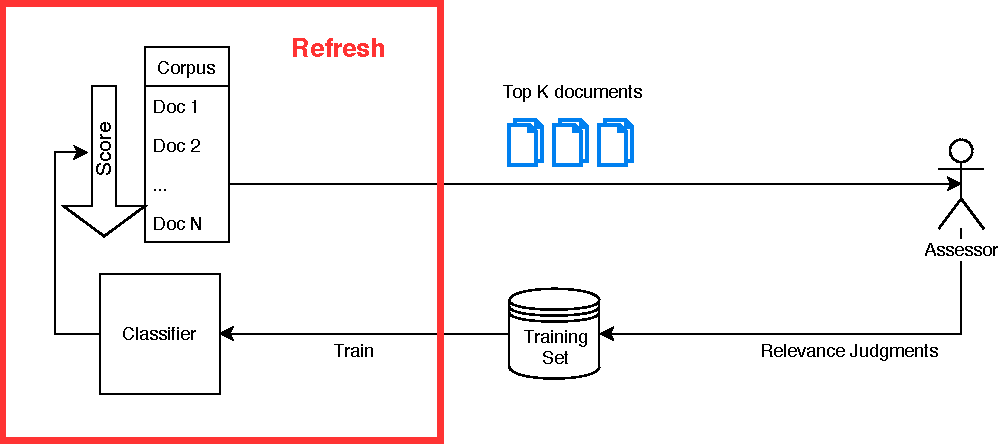
\includegraphics[width=1.0\textwidth]{talk_sigir/animation/3.pdf}
 \caption{A simplified view of the relevance feedback loop in Continuous Active
 Learning}
 \label{fig:calloop}
\end{figure}


The organizers of the TREC 2015 Total Recall Track distributed the Baseline
Model Implementation (BMI) of AutoTAR as a virtual machine. The implementation
was a collection of C++ programs invoked and orchestrated using few BASH
scripts.  In BMI, documents are represented as a vector of unigram tf-idf
features which are used for training the classifier and calculating relevance
likelihood scores. BMI relies on
sofia-ml\footnote{https://code.google.com/archive/p/sofia-ml/}
\cite{sculley2010combined} to train a logistic regression classifier using the
\textit{logreg-pegasos} learner with $200000$ iterations of \textit{roc}
sampling. A training iteration involves randomly sampling a relevant and a
non-relevant document from the training set, computing the loss and adjusting
the classifier weights accordingly. The relevance likelihood score for any
document is obtained by computing the dot product of the classifier weights and
document feature vector.

\section{Related Work}

The Baseline Model Implementation (BMI) was made available to the participants
by the organizers of the Total Recall Track in TREC 2015. We take a look at few
approaches of participants which are relevant to our interest.

The UvA.ILPS team~\cite{van2015university} modified the way batch sizes were
set in BMI. They started with a batch size of 100. After a batch was assessed, the
batch size was set to some value proportional to the number of relevant
documents assessed in the previous batch.

The Webis team~\cite{hagen2015webis} used BM25 using the topic description as query to get an
initial set of documents which were used to train a SVM classifier. The batch size of
to-be-assessed-documents was initially set to 32. After every iteration, it was
either halved, doubled, or untouched depending on the ratio of documents
assessed relevant and non-relevant. Another run submitted by this team used
keyphrase extraction from document assessed as relevant to perform ad-hoc
searches at every step and use it to enhance the SVM classifier.

The TUW team~\cite{lupu2015tuw} tweaked the term weighting in the document feature vectors
used by the BMI. In another run, they used all the learners available in
sofia-ml separately and then used voting to select relevant documents.


There is a vast literature which separately addresses efficiency and scalability
of various steps in the AutoTAR algorithm. Online learning algorithms can
significantly improve the running times of the training step. Such algorithms
have been investigated in detail for spam
filtering~\cite{sculley2007relaxed,cormack2007online,sculley2007online}.
\citet{cormack2011efficient} proposed an online logistic regression based spam filter for large
datasets. \citet{crammer2006online} proposed a SVM-based
Passive-Aggressive algorithm for online binary
classification. Both of these online learning methods
make a prediction for an incoming training examples and depending on the ground
truth, updates the classifier weights.

% In CAL, fetching a set of documents for review requires scoring of all the
% documents in the collection and presenting the top few documents to the assessor.
